\documentclass[12pt]{article}

% \usepackage[utf8]{inputenc}
% \usepackage[catalan]{babel}
% SILENCE THE WARNINGS!
%\usepackage{silence}


% tufte-book ja inclou el paquet geometry, i per tant només
% cal canviar alguns paràmetres amb \geometry
\geometry{a4paper, top=25mm, bottom=30mm, inner=20mm, outer=70mm}
\setlength{\marginparwidth}{50mm}  % Adjust margin for sidenotes
%\geometry{margin=3cm,headsep=0.25in}
%\geometry{showframe}% for debugging purposes -- displays the margins
% The units package provides nice, non-stacked fractions and better spacing
% for units.
%\usepackage{units}
%\usepackage{todonotes}

\usepackage{framed}
\usepackage{ifthen}
\usepackage{longtable}
\usepackage{fancyvrb}
\fvset{fontsize=\normalsize}
%\usepackage{cancel}

\usepackage[utf8]{inputenc}
\usepackage[catalan]{babel}
\usepackage{lmodern}
\usepackage{amsmath,amsthm,amsfonts,amssymb,amscd}
\usepackage{multirow,booktabs}
\usepackage[dvipsnames,table]{xcolor}
%\usepackage{fullpage}
\usepackage{lastpage}
\usepackage{graphicx}
%\setkeys{Gin}{width=\linewidth,totalheight=\textheight,keepaspectratio}
\graphicspath{{../figures/}}
\usepackage{enumitem}
\usepackage{fancyhdr}
\usepackage{mathrsfs}
\usepackage{wrapfig}
\usepackage{setspace}
\usepackage{calc}
\usepackage{multicol}
\usepackage{gensymb}



\usepackage[most]{tcolorbox}


\usepackage{cancel}
\usepackage[retainorgcmds]{IEEEtrantools}

%\newlength{\tabcont}
% \setlength{\parindent}{0.0in}
% \setlength{\parskip}{0.05in}
%\usepackage{empheq}
% es recomana que mdframed es carregui després de xcolor
\usepackage[framemethod=TikZ]{mdframed}
\mdfdefinestyle{caixa}{leftmargin=1cm,innerrightmargin=0.5cm, linecolor=blue}

\usepackage{changepage}







\usepackage{url}
  \let\oldurl\url
\usepackage{hyperref}
  \let\linkurl\url
  \let\url\oldurl
  
%\chemsetup[chemformula]{format=\sffamily}

%\setatomsep{2em}
%\setdoublesep{.6ex}
%\setbondstyle{semithick}
\colorlet{shadecolor}{orange!15}
\parindent 0in
\parskip 12pt


\theoremstyle{definition}
\newtheorem{defn}{Definition}
\newtheorem{reg}{Rule}
\newtheorem{exer}{Exercise}
\newtheorem{note}{Note}
%\RequirePackage{mathrsfs}
%\RequirePackage[psamsfonts]{amsfonts} %for Y&Y BSR AMS fonts
\RequirePackage{amsmath,amsfonts,amsthm,amssymb}
\RequirePackage{setspace}
\RequirePackage{fancyhdr}
\RequirePackage{lastpage}
\RequirePackage{extramarks}
%\RequirePackage{chngpage}
\RequirePackage{soul}
%\RequirePackage{graphicx,float,wrapfig}
%\RequirePackage{pgf,tikz}
%\usetikzlibrary{arrows,automata}
%\RequirePackage{pstricks}
%\RequirePackage[text]{amsthm}
%\RequirePackage{array}
%\RequirePackage{amscd}
%\RequirePackage{array}\RequirePackage{dcolumn}

\newcommand{\emx}[1]{{\em{#1}\/}}
\newcommand{\abin}{{\it ab initio}}
\newcommand{\bs}{\boldsymbol}
%\newcommand{\citepnum}{\citep}
\newcommand{\dGo}{\ensuremath{\Delta G_0}}
\newcommand{\dG}[2]{\ensuremath{\Delta G_{\rm #1}^{\rm #2}}}
\newcommand{\dX}[3]{\ensuremath{\Delta #1_{\rm #2}^{\rm #3}}}
\newcommand{\ddgo}[1]{\ensuremath{\Delta \Delta G_{\rm solv}^{\rm #1}}}
\newcommand{\ddgstarcat}{\ensuremath{\Delta \Delta g^{\ddagger}_{\rm cat}}}
\newcommand{\ddgstar}{\ensuremath{\Delta \dgstar}}
\newcommand{\ddgt}[2]{\ensuremath{\Delta \Delta G_{\rm solv}^{\rm #1, \rm #2}}}
\newcommand{\ddsstarprime}{\ensuremath{(\Delta \dsstar)'}}
\newcommand{\deltaepsel}{\ensuremath{\Delta \varepsilon_{\rm el}}}
\newcommand{\deltaeps}{\ensuremath{\Delta \varepsilon}}
\newcommand{\dgab}[2]{\ensuremath{\Delta g_{\rm #1}^{\rm #2}}}
\newcommand{\dga}[1]{\ensuremath{\Delta g_{\rm #1}}}
\newcommand{\dgb}[1]{\ensuremath{\Delta g^{\rm #1}}}
\newcommand{\dgcage}{\ensuremath{\Delta g_{\rm cage}}}
\newcommand{\dgcat}{\ensuremath{\Delta g_{\rm cat}}}
\newcommand{\dgsoltsatsa}{\ensuremath{\dgsol (\rm TSA)_{\rm TSA}}}
\newcommand{\dgsoltstsa}{\ensuremath{\dgsol (\rm TS)_{\rm TSA}}}
\newcommand{\dgsoltsts}{\ensuremath{\dgsol (\rm TS)_{\rm TS}}}
\newcommand{\dgsol}{\ensuremath{\Delta G_{\rm sol}}}
\newcommand{\dgstarcage}{\ensuremath{\dgstar_{\rm cage}}}
\newcommand{\dgstarcat}{\ensuremath{\dgstar_{\rm cat}}}
\newcommand{\dgstarw}{\ensuremath{\dgstar_{\rm w}}}
\newcommand{\dgstar}{\ensuremath{\Delta g^{\ddagger}}}
\newcommand{\dgw}{\ensuremath{\Delta g_{\rm w}}}
\newcommand{\dg}[2]{\ensuremath{\Delta g_{\rm #1}^{\rm #2}}}
\newcommand{\dino}{\texttt{DINO}}
\newcommand{\dsstarcageprime}{\ensuremath{(\dsstarcage)'}}
\newcommand{\dsstarcage}{\ensuremath{\dsstar_{\rm cage}}}
\newcommand{\dsstarcatprime}{\ensuremath{(\dsstarcat)'}}
\newcommand{\dsstarcat}{\ensuremath{\dsstar_{\rm cat}}}
\newcommand{\dsstarwprime}{\ensuremath{(\dsstarw)'}}
\newcommand{\dsstarw}{\ensuremath{\dsstar_{\rm w}}}
\newcommand{\dsstar}{\ensuremath{\Delta S^{\ddagger}}}
\newcommand{\eg}{{\it e.g.}}
\newcommand{\etal}{{\it et al.}}
\newcommand{\gamess}{\texttt{GAMESS}}
\newcommand{\gauss}{\texttt{GAUSSIAN} 98}     
\newcommand{\golpe}{\texttt{GOLPE}}                                             
\newcommand{\grid}{\texttt{GRID}}
\newcommand{\ie}{{\it i.e.}}
\newcommand{\ith}{{\it i}$^{\rm th}$\ }
\newcommand{\kbt}{\ensuremath{k_{\rm B} T}}
\newcommand{\kb}{\ensuremath{k_{\rm B}}} 
\newcommand{\kcage}{\ensuremath{k_{\rm cage}}}
\newcommand{\kcatkm}{\ensuremath{k_{\rm cat}/K_{\rm M}}}
\newcommand{\kcat}{\ensuremath{k_{\rm cat}}}
\newcommand{\km}{\ensuremath{{\rm\, kcal \, mol}^-1}}
\newcommand{\knon}{\ensuremath{k_{\rm non}}}
\newcommand{\kw}{\ensuremath{k_{\rm w}}}
\newcommand{\mepsim}{\texttt{MEPSIM}}
\newcommand{\mgp}[1]{\marginpar{\scriptsize{#1}}}
\newcommand{\mipsim}{\texttt{MIPSIM}}
\newcommand{\mola}{\texttt{MOLARIS}}
\newcommand{\msms}{\texttt{MSMS}}
\newcommand{\pdras}{p21$^{\rm ras}$}
\newcommand{\rgran}{\ensuremath{\mathbb{R}}}
\newcommand{\rx}[2]{\ensuremath{#1_{\rm #2}}}
\newcommand{\vs}{{\it vs.}}
\newcommand{\z}[1]{\ensuremath{\mathbf{#1}}} 
\newcommand{\composed}[2]{#1\mathbin\circ #2}
\newcommand{\wrt}[1]{{\mbox{\scriptsize w.r.t. \( #1 \)} }}
\newcommand{\polyspace}{\mathcal{P}}
\newcommand{\matspace}{\mathcal{M}}
\newcommand{\C}{\mathbb{C}}
\newcommand{\N}{\mathbb{N}}
\newcommand{\Q}{\mathbb{Q}}
\newcommand{\Z}{\mathbb{Z}}
\renewcommand{\Re}{\mathbb{R}}
\newcommand{\rtres}{\ensuremath{\Re^3}}
\newcommand{\union}{\cup}
\newcommand{\dotprod}{\cdot}
%\newcommand*\pkg[1]{\textsf{#1}}

\newcommand{\trans}[1]{{#1}^{\ensuremath{\mathsf{T}}}} % transpose
\newcommand{\nbyn}[1]{\ensuremath{#1 \! \times \! #1 }}
\newcommand{\nbym}[2]{#1 \! \times \! #2 }       % Use in math mode.
\newcommand{\cat}[2]{#1\!\mathbin{\raise.6ex\hbox{\( {}^\frown \)}}\!#2}
\newcommand{\generalmatrix}[3]{ %arg1: low-case letter, arg2: rows, arg3: cols
               \left(
                  \begin{array}{cccc}
                    #1_{1,1}  &#1_{1,2}  &\ldots  &#1_{1,#2}  \\
                    #1_{2,1}  &#1_{2,2}  &\ldots  &#1_{2,#2}  \\
                              &\vdots                         \\
                    #1_{#3,1} &#1_{#3,2} &\ldots  &#1_{#3,#2}
                  \end{array}
               \right)  }
\newcommand{\colvec}[1]{\begin{pmatrix} #1 \end{pmatrix}}
\newcommand{\pr}[1]{\ensuremath{\mathrm{Pr}(#1)}}
\newcommand{\rep}[2]{ {\rm Rep}_{#2}(#1) }
\newcommand{\mapsunder}[1]{\stackrel{#1}{\longmapsto}}
\newcommand{\map}[3]{\mbox{$#1\colon #2\to #3$}}
\newcommand{\identity}{\mbox{id}}
\newcommand{\stdbasis}{{\cal E}} 
\newcommand{\sequence}[1]{ \langle#1\rangle } 
\newcommand{\spacer}{\rule[-3mm]{0mm}{8mm}}
\newcommand{\email}[1]{\url{#1}}
\newcommand{\zero}{\vec{0}}
\newcommand{\proj}[2]{\mbox{proj}_{#2}({#1}) }
%\AtBeginDocument{\newlength{\heightofcdot}
%\newlength{\widthofcdot}
%\settoheight{\heightofcdot}{$\cdot$}
%\settowidth{\widthofcdot}{$\cdot$}
%\newsavebox{\dotprodcircle}       
%\savebox{\dotprodcircle}{\includegraphics{dotprod.1}} 
%\newcommand{\dotprod}{\mathbin{\raisebox{.5\heightofcdot}{%
%          \makebox[\widthofcdot]{$\smash{\usebox{\dotprodcircle}}$}}}}}
\newcommand{\spanof}[1]{\relax [#1\relax ]} % no optional argument!
\newcommand{\set}[1]{\mbox{$\{#1\}$}} \newcommand{\suchthat}{\bigm|}
\newcommand{\deter}[1]{ \mathchoice{\left|#1\right|}{|#1|}{|#1|}{|#1|} }
\newcommand{\secuence}[1]{ \langle#1\rangle }  
\newcommand{\basis}[2]{\secuence{\vec{#1}_1,\ldots,\vec{#1}_{#2}}}



%--------linsys
%  Use as \begin{linsys}{3}
%           x &+ &3y &+ &a &= &7 \\
%           x &- &3y &+ &a &= &7
%         \end{linsys}
% Remark: TeXbook pp. 167-170 says to put a medmuskip around a +; and that's
% 4/18-ths of an em.  Why does 2/18-ths of an em work?  I don't know, but
% comparing to a regular displayed equation suggests it is right.
% (darseneau says LaTeX puts in half an \arraycolsep.)
\newenvironment{linsys}[2][m]{%
\setlength{\arraycolsep}{.1111em} % p. 170 TeXbook; a medmuskip
\begin{array}[#1]{@{}*{#2}{rc}r@{}}
}{%
\end{array}}


%\newtheorem{teorema}{Teorema}
%\newtheorem{exercici}{Exercici}
%\newtheorem{definicio}{Definici\'o}
%\newtheorem{theorem}{Theorem}
\newtheorem{exercise}{Exercise}
%\newtheorem{definition}{Definition}

\newcounter{EXMP}
\newenvironment{EXMP}[1][]{\definecolor{shadecolor}{rgb}{0.6,0.6,0.6}
							\begin{shaded}\refstepcounter{EXMP}\par\medskip\noindent%
   							\textbf{EXAMPLE~\theEXMP. #1} \rmfamily}
   							{\end{shaded}\medskip}

\newcounter{BOXT}
\newenvironment{BOXT}[1][]{\definecolor{shadecolor}{rgb}{0.8,0.8,0.8}
							\begin{shaded}\refstepcounter{BOXT}\par\medskip\noindent%
   							\textbf{BOX~\theBOXT. #1} \rmfamily}
   							{\end{shaded}\medskip}

\parskip 4mm


\usepackage{makeidx}
\makeindex




%\setcounter{section}{-1}

\theoremstyle{definition}
\newtheorem{thm}{Theorem}
\newtheorem{dfn}{Definition}
\newtheorem{lem}{Lemma}
\newtheorem{prp}{Proposition}





%%%%%%%%%%%%%%%%%%%
% ANGLÈS
%%%%%%%%%%%%%%%%%%%

% \newcommand{\problemName}{}%
% \newcounter{problemCounter}%
% \newenvironment{problem}[1][Problem \arabic{problemCounter}]%
% 	{\stepcounter{problemCounter}%
% 		\renewcommand{\problemName}{#1}%
% 		\section*{\problemName}%
% 		\nobreak\extramarks{\problemName}{\problemName continued on next page\ldots}\nobreak%
% 		\nobreak\extramarks{\problemName (continued)}{\problemName continued on next page\ldots}\nobreak}%
% 	{\nobreak\extramarks{\problemName (continued)}{\problemName continued on next page\ldots}\nobreak%
% 		\nobreak\extramarks{\problemName}{}\nobreak}%

\newenvironment{example}{ % 
	\definecolor{shadecolor}{rgb}{0.8,1.0,0.8} %
	\begin{shaded} %
	\textcolor{OliveGreen}{\bf Example\\}%
} % 
{ %	
	\end{shaded}
} %


\newenvironment{introduction}{ % 
	\definecolor{shadecolor}{rgb}{1.0,1.0,0.8} %
	\begin{shaded} %
	% \textcolor{BrickRed}{\bf Introduction\\}%
} % 
{ %	
	\end{shaded}
} %


%%%%%%%%%%%%%%%%%%%
% CATALÀ
%%%%%%%%%%%%%%%%%%%
\newtheorem{teorema}{theorem}
\newenvironment{definicio}{ % 
	\definecolor{shadecolor}{rgb}{0.9,1.0,0.8} %
	\begin{shaded} %
	\textcolor{OliveGreen}{\bf Definicio\\}%
} % 
{ %	
	\end{shaded}
} %

%veure http://en.wikibooks.org/wiki/LaTeX/Advanced_Topics

\newcommand{\doccmd}[1]{\texttt{\textbackslash#1}}% command name -- adds backslash automatically
\newcommand{\docopt}[1]{\ensuremath{\langle}\textrm{\textit{#1}}\ensuremath{\rangle}}% optional command argument
\newcommand{\docarg}[1]{\textrm{\textit{#1}}}% (required) command argument
\newenvironment{docspec}{\begin{quote}\noindent}{\end{quote}}% command specification environment
\newcommand{\docenv}[1]{\textsf{#1}}% environment name
\newcommand{\docpkg}[1]{\texttt{#1}}% package name
\newcommand{\doccls}[1]{\texttt{#1}}% document class name
\newcommand{\docclsopt}[1]{\texttt{#1}}% document class option name
\newcommand{\logos}{%
\begin{figure}

\includegraphics{FCTE}
\end{figure}
}

% margins
% \topmargin=-0.45in      %
% \evensidemargin=0in     %
% \oddsidemargin=0in      %
% \textwidth=6in        %
% \textheight=8.5in       %
% \headsep=0.25in         %

% header and footer
\pagestyle{fancy}       %
\chead{}                %
\makeatletter
\fancyfoot[R]{%
   % We want italics
   \itshape
   % The chapter number only if it's greater than 0
   \ifnum\value{chapter}>0 \@chapapp\ \thechapter. \fi
   % The chapter title
   \leftmark}
\makeatother

%\lfoot{
\includegraphics[trim=-5cm 0 0 -3cm,width=0.4\textwidth]{FCTE}}      
\lfoot{\raisebox{-0.5cm}[0pt][0pt]{
\includegraphics[width=3cm]{FCTE}}} 

\cfoot{}        %
\renewcommand\headrulewidth{0.4pt}   %
\renewcommand\footrulewidth{0.4pt}   %

\usepackage{chemfig,chemmacros,chemnum}
\chemsetup[reactions]{
    before-tag = R,
    tag-open = [ , tag-close = ]
}
\chemsetup{
  formula = chemformula , % or mhchem
  modules = thermodynamics
}
\setchemfig{scale=0.3}
\renewcommand*\printatom[1]{\ensuremath{\mathsf{#1}}}
\usepackage{chemformula}

\usepackage{siunitx}

% Definició d'unitats personalitzades per al sistema imperial
\DeclareSIUnit\inch{in}
\DeclareSIUnit\foot{ft}
\DeclareSIUnit\atm{atm}
\DeclareSIUnit\oz{oz}
\DeclareSIUnit\ounce{oz}
\DeclareSIUnit\pound{lb}
\DeclareSIUnit\ton{t}

\DeclareSIUnit\cubicinch{\inch\cubed}
\DeclareSIUnit\cubicfoot{\foot\cubed}
\DeclareSIUnit\gallon{gal}
\DeclareSIUnit\psi{psi}
\DeclareSIUnit\inchHg{inHg}
\DeclareSIUnit\dyn{dynes}
\DeclareSIUnit\torr{Torr}
\DeclareSIUnit\Torr{Torr}
\DeclareSIUnit\inch{in}
\DeclareSIUnit\foot{ft}
\DeclareSIUnit\atm{atm}
\DeclareSIUnit\oz{oz}
\DeclareSIUnit\ounce{oz}
\DeclareSIUnit\pound{lb}
\DeclareSIUnit\ton{t}
\DeclareSIUnit\fah{F}
\DeclareSIUnit{\degreeFahrenheit}{\unit{\degree}F}
\newcommand{\degC}{\degreeCelsius}
\newcommand{\degF}{\degreeFahrenheit}




% \usepackage{chemformula}
% \usepackage{chemmacros}
% \chemsetup[reactions]{
%     before-tag = R,
%     tag-open = [ , tag-close = ]
% }
% \usepackage{siunitx}
% % Definició d'unitats personalitzades per al sistema imperial
% \DeclareSIUnit\inch{in}
% \DeclareSIUnit\foot{ft}
% \DeclareSIUnit\atm{atm}
% \DeclareSIUnit\oz{oz}
% \DeclareSIUnit\ounce{oz}
% \DeclareSIUnit\pound{lb}
% \DeclareSIUnit\ton{t}
% \DeclareSIUnit\torr{Torr}

% \DeclareSIUnit\cubicinch{\inch\cubed}
% \DeclareSIUnit\cubicfoot{\foot\cubed}
% \DeclareSIUnit\gallon{gal}
% \DeclareSIUnit\psi{psi}
% \DeclareSIUnit\inchHg{inHg}
% \DeclareSIUnit\dyn{dynes}

\DeclareSIUnit{\degreeFahrenheit}{\unit{\degree}F}
\newcommand{\degC}{\degreeCelsius}
\newcommand{\degF}{\degreeFahrenheit}
% mates
\usepackage{cancel}
\usepackage{graphicx}
\graphicspath{{../figures/}}

\usepackage{framed}
\newcounter{myc}
%environment for exercises in the class notes
\newenvironment{exr}[1]{ % 
    \addtocounter{myc}{1}
	\definecolor{shadecolor}{rgb}{0.9,1.0,0.8} %
	\begin{shaded} %
	\textcolor{OliveGreen}{\bf Exercici \arabic{myc}. {\bf #1}\\}%
} % 
{ %	
	\end{shaded}
} %
\usepackage[dvipsnames,table]{xcolor}
\newenvironment{qst}{ % 
    \addtocounter{myc}{1}
	\definecolor{shadecolor}{rgb}{0.9,1.0,0.8} %
	\begin{shaded} %
	\textcolor{OliveGreen}{\bf Exercici \arabic{myc}\\}%
} % 
{ %	
	\end{shaded}
} %

%%%%%%%%%%%%%%%%%%%%%%%%%%%%%%%%%%%%%%%%%
%%%%%%%%%%%%%%%%%%%%%%%%%%%%%%%%%%%%%%%%%
% lecturer or student text
% in principle the lecturer text includes some examples to be done in the c lass
\usepackage{ifthen}
\newboolean{LECT}
\setboolean{LECT}{true}
%%%%%%%%%%%%%%%%%%%%%%%%%%%%%%%%%%%%%%%%%
%%%%%%%%%%%%%%%%%%%%%%%%%%%%%%%%%%%%%%%%%

\newenvironment{lect}{ % 
	% \definecolor{shadecolor}{rgb}{1.0,0.8,0.8} %
	% \begin{shaded} %
	% \textcolor{BrickRed}{\bf Resultat\\}%

} % 
{ %	
	% \end{shaded}
} %

\newcommand{\lct}[1]{\ifthenelse{\boolean{LECT}}{\begin{lect} #1 \end{lect}}{}}

% header and footer
\usepackage{fancyhdr}

\pagestyle{fancy}       %
\lhead{\bf Química GEA-17UV}                %
\chead{}                %
\rhead{\bf Grau d'Enginyeria de l'Automoció}                %
\fancyfoot[R]{\thepage}
\lfoot{Exercicis resolts}
\cfoot{\today}                %

\usepackage[backend=bibtex,style=numeric]{biblatex} 

\title{Química Enginyeria de l'Automoció: Exercicis}
\date{Curs 2024-2025\\\small{(darrera actualització: \today)}}
\author{Jordi Vill\`a i Freixa (jordi.villa@uvic.cat)}
\addbibresource{../Teoria/QuimAutom.bib}
\begin{document}
\maketitle
\tableofcontents
\section{Els gasos i el seu comportament}
\begin{exr}
    Un conductor comprova la pressió dels pneumàtics pel matí aviat, quan la temperatura és de 15\si\degreeCelsius, i és de 1.3$\times$10$^5$ Pa. Al migdia la temperatura és 15 graus més elevada. Quina és la pressió dels pneumàtics ara?.
    \end{exr}
	
    \begin{exr}
        Dalt de l'Everest, la pressió atmosfèrica és de 0,33 atm i la temperatura de 50 sota zero. Quina és la densitat de l'aire si en CN és de 1.29\si{\gram\per\deci\meter\tothe{3}}?.
        \end{exr}
    \lct{


Sabem que la densitat de l'aire en condicions normals (CN) és:

\[
\rho_{\text{CN}} = \SI{1.29}{\gram\per\deci\meter\cubed}
\]

Les condicions a dalt de l’Everest són:

\begin{itemize}
    \item Pressió atmosfèrica: \( P = \SI{0.33}{\atm} \)
    \item Temperatura: \( T = \SI{-50}{\celsius} = \SI{223}{\kelvin} \)
    \item Condicions normals (CN):
    \begin{itemize}
        \item Pressió normal: \( P_{\text{CN}} = \SI{1}{\atm} \)
        \item Temperatura normal: \( T_{\text{CN}} = \SI{273}{\kelvin} \)
    \end{itemize}
\end{itemize}

Sabem que la densitat d'un gas està relacionada amb la pressió i la temperatura segons l'expressió:

\[
\frac{\rho}{\rho_{\text{CN}}} = \frac{P}{P_{\text{CN}}} \times \frac{T_{\text{CN}}}{T}
\]

Aïllant \( \rho \):

\[
\rho = \rho_{\text{CN}} \times \frac{P}{P_{\text{CN}}} \times \frac{T_{\text{CN}}}{T}
\]

Substituïm els valors donats:

\[
\rho = (\SI{1.29}{\gram\per\deci\meter\cubed}) \times \frac{\SI{0.33}{\atm}}{\SI{1}{\atm}} \times \frac{\SI{273}{\kelvin}}{\SI{223}{\kelvin}}=\SI{0.52}{\gram\per\deci\meter\cubed}
\]

    }	
\begin{exr}
    Calcular el volum molar d'un gas ideal a condicions normals (1 atm i 0\si\degreeCelsius).
    \end{exr}
\begin{exr}
    Quant gas hi ha en una mostra de volum \qty{0.5}{\deci\meter\tothe{3}}, a \qty{80}{\degC} i \qty{800}{\torr} de pressió?
    \end{exr}

\begin{exr}{}
Pots calcular el volum ocupat per molècula en un gas ideal a CN?. Es troben dues molècules molt freqüentment en un gas a baixa pressió?
\end{exr}

    \begin{exr}
        Si a CN la densitat d'un gas ideal és de \qty{2.62}{\gram\per\deci\meter\tothe{3}}, quina és la seva massa molar? i quina densitat tindrà a 300 K i \qty{2.4e5}{\pascal} 2.4$\times$10$^5$ Pa?
        \end{exr}


        
\begin{exr}{}
Quant gas hi ha en una mostra de volum 0.5 dm$^3$, a 80 graus Celsius i 800 Torr de pressió?.
\end{exr}

\begin{exr}
Què passa segons l'Equació de van der Waals si la pressió es fa propera a zero o bé la temperatura es fa molt gran per a un gas real?   La figura mostra el factor de compressibilitat per a un mateix gas a diferents temperatures
\begin{center}        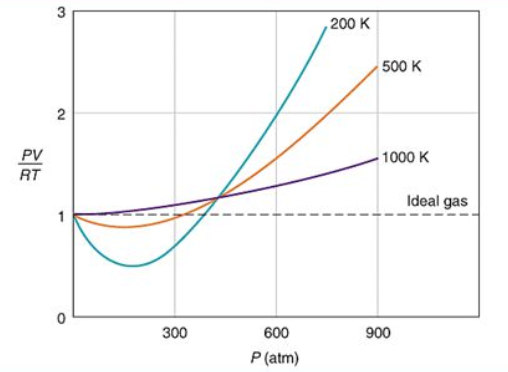
\includegraphics[scale=1.0]{FactorCompressT.png}
\end{center}
\end{exr}
\begin{exr}{Comparativa TCG per a \ch{H2} i \ch{He}}
Es prepara una mescla de gasos d'hidrogen (\ch{H2}) i heli (\ch{He}) tal que les molècules de cada gas produeixin el mateix nombre de col·lisions amb la paret per unitat de temps. Determinem quin gas té la concentració més alta.
\end{exr}
\lct{
\textbf{Consideració com a gasos ideals}

L'energia cinètica translacional d'un mol de gas és 
\[\left<E_c\right>=N_0 \frac{m <c^2>}{2}=\frac{3}{2} RT\]
on $M=N_0m$ és la massa molecular del gas en \si{\kilogram\per\mole}. 

Per tant, la velocitat quadràtica mitjana és:

\begin{equation}
    c_{\text{rms}} = \sqrt{\frac{3RT}{M}}
\end{equation}
Com que la taxa de col·lisions amb la paret és proporcional a $n v_{\text{rms}}$, imposem la condició d'igualtat:
\begin{equation}
    n_{\ch{H2}} \cdot \sqrt{\frac{3RT}{M_{\ch{H2}}}} = n_{\ch{He}} \cdot \sqrt{\frac{3RT}{M_{\ch{He}}}}
    \label{Eq:igualtat}
\end{equation}

A l'Eq. \ref{Eq:igualtat} hem usat que el nombre de col·lisions és proporcional al producte del nombre de molècules per la velocitat promig a la que es mouen. Per a entendre-ho, imaginem un cas simple de tres pilotes que es mouen a 10 m/s en línia recta i fan rebots entre dues parets d'una habitació. Si l'habitació fa 10 metres de llarg, en 10 segons cada pilota haurà tocat les parets 10 cops. Per tant, el nombre de xocs haurà estat 30.
Si enlloc de 3 pilotes en tinguéssim 10 que es mouen a 3 metres per segon, haurien tocat les parets també 30 cops (cada pilota, en 10 segons, hauria recorregut 30 metres, i per tant hauria xocat 3 cops contra les parets; com que tenim 10 pilotes, el nombre total de xocs és 30).

Substituint masses moleculars $M_{\ch{H2}} = 2$ g/mol i $M_{\ch{He}} = 4$ g/mol a l'Eq. \ref{Eq:igualtat}:
\begin{equation}
    n_{\ch{H2}} \cdot \sqrt{\frac{1}{2}} = n_{\ch{He}} \cdot \sqrt{\frac{1}{4}}
\end{equation}
\begin{equation}
    n_{\ch{H2}} \cdot \frac{1}{\sqrt{2}} = n_{\ch{He}} \cdot \frac{1}{2}
\end{equation}
Resolent per $n_{\ch{H2}}$:
\begin{equation}
    n_{\ch{H2}} = \frac{n_{\ch{He}}}{\sqrt{2}}
\end{equation}
Per tant, la concentració de $\ch{H2}$ ha de ser més baixa que la de $\ch{He}$.
És a dir, si volem igualar les vegades que xoquen contra les parets d'un volum les molècules d'He i d'H2, hem de plantejar l'expressió d'igualtat de l'Eq. \ref{Eq:igualtat} on la partícula amb més massa, pel fet d'anar més lenta, necessitarà més partícules en moviment, és a dir, més concentració.

%\\[10pt]
\textbf{Consideració com a gasos no ideals}

Si considerem gasos reals, hem de corregir la velocitat mitjana tenint en compte el factor de compressibilitat $Z$:
\begin{equation}
    v_{\text{rms}} = \sqrt{\frac{3ZRT}{M}}
\end{equation}
Ara, l'Eq. \ref{Eq:igualtat} es transforma en:
\[
    n_{\ch{H2}} \cdot \sqrt{\frac{3Z_{\ch{H2}}RT}{M_{\ch{H2}}}} = n_{\ch{He}} \cdot \sqrt{\frac{3Z_{\ch{He}}RT}{M_{\ch{He}}}}
\]
d'on
\[
    \frac{n_{\ch{H2}}}{n_{\ch{He}}}=\sqrt{\frac{\frac{3Z_{\ch{He}}RT}{M_{\ch{He}}}}{\frac{3Z_{\ch{H2}}RT}{M_{\ch{H2}}}}}
    =\sqrt{\frac{Z_{\ch{He}}M_{\ch{H2}}}{Z_{\ch{H2}}M_{\ch{He}}}}
\]
A pressions altes, $Z_{\ch{H2}} > Z_{\ch{He}}$ per les interaccions intermoleculars més fortes d'hidrogen (veure la Fig. Gasos-\ref{Gasos-fig:FactorCompress}), la qual cosa encara reforça més la diferència entre les concentracions de les dues expècies químiques. 
}


\begin{exr}{Pressions parcials aire}
La composició percentual, en massa, de l'aire sec al nivell del mar és, aproximadament, \ch{N2}/\ch{O2}/\ch{Ar}=75.5/23.2/1.3. 
Quina és la pressió parcial de cada component quan la pressió total és 1.20 atm?.
\end{exr}
\lct{
En 100gr d'aire tindrem 75.5, 23.2 i 1.3 gr de \ch{N2}, \ch{O2} i \ch{Ar}, respectivament. Podem calcular la seva fracció molar calculant el número de mols de cadascun i dividint pel total. Després, només cal multiplicar per la pressió corresponent i sabrem la pressió parcial de cada component:

\[n_{\ch{N2}}=75.5 \cancel{g} \cdot \frac{1 mol}{28.02 \cancel{g}}=2.69 mol\]
\[n_{\ch{O2}}=23.2 \cancel{g} \cdot \frac{1 mol}{32.00 \cancel{g}}=0.725 mol\]
\[n_{\ch{Ar}}=1.3 \cancel{g} \cdot \frac{1 mol}{39.95 \cancel{g}}=0.033 mol\]

    \begin{tabular}{cccc}
      \hline
        & \ch{N2} & \ch{O2} & \ch{Ar} \\
      \hline
Fracció molar &	0.780 & 0.210 & 0.0096\\
Pressió parcial (nivell del mar)/atm & 0.780 & 0.210 & 0.0096\\
Pressió parcial ($P_T=1.20$atm))/atm & 0.936 & 0.252 & 0.012\\
      \hline
    \end{tabular}
}
 % Dalton
\begin{exr}
Una barreja de metà \ch{CH4} i d'acetilè \ch{C2H2} ocupava un cert volum a una pressió total de 63 mmHg. La mostra es va cremar a \ch{CO2} i \ch{H2O}. Se'n va recollir el \ch{CO2} en el mateix volum inicial i la mateixa temperatura inicial, i es va veure que la seva pressió era de 96 mmHg. Quina era la fracció de metà a la mescla de gasos inicials?
\end{exr}
\lct{
Definim $x$ com la fracció molar de metà (\ch{CH4}) i $y$ com la fracció molar d’acetilè (\ch{C2H2}):  
        \[
        x + y = 1
        \]
   
    Les reaccions de combustió són:
    
    \begin{align}
        \ch{CH4 + 2 O2 -> CO2 + 2 H2O}  & \quad \text{(1 mol de \ch{CH4} produeix 1 mol de \ch{CO2})} \\
        \ch{C2H2 + 5/2 O2 -> 2 CO2 + H2O}  & \quad \text{(1 mol de \ch{C2H2} produeix 2 mols de \ch{CO2})}
    \end{align}
    
    Si tenim un nombre total de mols $n$, llavors:
    
    \begin{itemize}
        \item Mols de metà: $xn$
        \item Mols d'acetilè: $yn$
    \end{itemize}
    
    Els mols de \ch{CO2} formats són:
    
    \[
    n_{\ch{CO2}} = xn + 2yn
    \]
     
    Com que el volum i la temperatura es mantenen constants, segons la llei dels gasos ideals la pressió és directament proporcional als mols:
      
    Així:
    
    \[
    P_{\ch{CO2}} = (xn + 2yn) \cdot \frac{P_{\text{total}}}{n}
    \]
    
    Substituint els valors donats:
    
    \[
    96 = (x + 2y) \cdot 63
    \]
    
   d'on
    
    \[
    x + 2y = \frac{32}{21}
    \]
    
   Ara ja podem resoldre el sistema:
    
    \begin{align}
        x + y &= 1 \\
        x + 2y &= \frac{32}{21}
    \end{align}
    
    i obtenim   
    \[
    x = 1 - \frac{11}{21} = \frac{10}{21}
    \]
    
    Per tant, la fracció de metà en la mescla inicial és:
    
    \[
    \frac{10}{21} \approx 0.476 \quad \text{o} \quad 47.6\%
    \]
}

\begin{exr}{Fòrmula molecular d'un compost gasós}
    Un compost gasós que se sap que conté només carboni, hidrogen i nitrogen es barreja amb el volum d'oxigen exactament necessari per a la seva combustió completa a \ch{CO2}, \ch{H20} i \ch{N2}. La combustió de 9 volums de la mescla gasosa produeix 4 volums de \ch{CO2}, 6 volums de vapor d'aigua i 2 volums de \ch{N2}, tots a la mateixa temperatura i pressió.

    Quants volums d'oxigen es necessiten per a la combustió? Quina és la fórmula molecular del compost?
\end{exr}

\lct{

El compost gasós conté carboni (C), hidrogen (H) i nitrogen (N). Es barreja amb oxigen suficient per a la combustió completa, donant com a productes diòxid de carboni (\(\ch{CO2}\)), aigua (\(\ch{H2O}\)) i nitrogen molecular (\(\text{N}_2\)).

Es donen les següents dades:
\begin{itemize}
    \item Volum de la mescla gasosa: 9 volums
    \item Volum de \(\ch{CO2}\) produït: 4 volums
    \item Volum de \(\ch{H2O}\) produït: 6 volums
    \item Volum de \(\text{N}_2\) produït: 2 volums
\end{itemize}

Sigui la fórmula del compost:
\[
C_xH_yN_z
\]

L'equació de combustió és:
\[
C_xH_yN_z + \ch{O2} \rightarrow a C\ch{O2} + b \ch{H2O} + c N_2
\]

Per la conservació dels àtoms:

- Carboni: \( x = a = 4 \Rightarrow x = 4 \)
- Hidrogen: \( y = 2b = 6 \Rightarrow y = 6 \)
- Nitrogen: \( z = 2c = 2 \Rightarrow z = 2 \)

Així, la fórmula del compost és:
\[
C_4H_6N_2
\]

Per trobar el volum d'oxigen utilitzat, considerem la combustió completa:

\[
C_4H_6N_2 + \ch{O2} \rightarrow 4 C\ch{O2} + 3 \ch{H2O} + N_2
\]

L'oxigen es consumeix en la formació de \(\ch{CO2}\) i \(\ch{H2O}\):

\[
\ch{O2} \text{ necessari} = \frac{(4 \times 2) + (3 \times 1)}{2} = \frac{8 + 3}{2} = 5.5 \text{ volums}
\]

Per tant, el volum d'oxigen necessari és **5.5 volums**.

}

\input{../Exercicis/ex_hidrogenacioEtile.tex}
\begin{exr}{Pressió parcial \ch{PCl5} en una mescla (adaptat de \cite{mahan_quimica_1997})}
    Una mostra de \ch{PCl5}, que pesa \SI{2.69}{\gram}, es va col·locar en un flascó d'\SI{1.00}{\litre} i es va evaporar completament a una temperatura de \SI{250}{\celsius}. La pressió observada a aquesta temperatura va ser \SI{1.00}{\atm}. Existeix la possibilitat que una part del \ch{PCl5} s'hagi dissociat d'acord amb l'equació:

\begin{reaction}
PCl5(g) -> PCl3(g) + Cl2(g)
\end{reaction}

Quines són les pressions parcials del \ch{PCl5}, \ch{PCl3} i \ch{Cl2} en aquestes condicions experimentals?
\end{exr}
\lct{
    La solució d'aquest problema implica diverses etapes. Per determinar si s'ha dissociat una part del \ch{PCl5}, calculem primerament la pressió que s'hauria observat si no s'hagués dissociat el \ch{PCl5}. Això es pot calcular a partir del nombre de mols de \ch{PCl5} utilitzats, juntament amb el volum i la temperatura del flascó. Com que el pes molecular del \ch{PCl5} és \SI{208}{\gram\per\mole}, el nombre de mols de \ch{PCl5} inicialment presents en el flascó és:

\[
n = \SI{2.69}{\gram}\cdot \frac{1\si{\mole}}{\SI{208}{\gram}} = 0.0129\si{\mole}.
\]

La pressió corresponent a aquest nombre de mols seria:

\[
P = \frac{nRT}{V} = \frac{(0.0129\si{\mole})(\SI{0.082}{\liter\atm\per\mole\per\kelvin})(\SI{523.15}{\kelvin})}{\SI{1.00}{\liter}} = \SI{0.553}{\atm}.
\]

Com que la pressió observada és superior a aquesta, s'ha de produir certa dissociació del \ch{PCl5}. Aplicant la llei de les pressions parcials, podem escriure:

\begin{equation}
P_{\ch{PCl5}} + P_{\ch{PCl3}} + P_{\ch{Cl2}} = P_t = \SI{1.00}{\atm}.
\label{eq:daltonpcl}
\end{equation}

Ara observem que:


Atès que es produeix un mol de \ch{PCl3} i un mol de \ch{Cl2} per cada mol de \ch{PCl5} dissociat,
\[
P_{\ch{Cl2}} = P_{\ch{PCl3}}, \quad P_{\ch{PCl5}} = \SI{0.553}{\atm} - P_{\ch{Cl2}}.
\]
i podem reescriure l'Equació \ref{eq:daltonpcl} com:

\[
\SI{0.553}{\atm} - P_{\ch{Cl2}} + P_{\ch{Cl2}} + P_{\ch{Cl2}} = \SI{1.00}{\atm}.
\]

Resolent, obtenim:

\[
P_{\ch{Cl2}} = \SI{0.447}{\atm},
\]

i

\[
P_{\ch{PCl3}} = \SI{0.447}{\atm}, \quad P_{\ch{PCl5}} = \SI{0.106}{\atm}.
\]
}

\begin{exr}{Airbag (adaptat de \cite{bowers_understanding_2014})}
    Els coixins de seguretat ({\em airbag}) dels cotxes s'inflen mitjançant una sèrie de reaccions químiques ràpides que produeixen gas en menys de \qty{0.04}{\second}. En les seves primeres versions, la reacció es basava en la descomposició de \ch{NaN3} (extremadament tòxic), seguida de dues reaccions addicionals per neutralitzar els subproductes perillosos. Les equacions químiques d'aquest procés són:  
 
    \begin{reactions}
        2 NaN3 &-> 2 Na + 3 N2 (g) "\label{reac:nan3}"\\
        10 Na + 2 KNO3 &-> K2O + 5 Na2O + N2 (g) "\label{reac:na}"\\
        K2O + Na2O + 2 SiO2 &-> K2SiO3 + Na2SiO3
    \end{reactions}

Un coixí de seguretat de conductor té un volum aproximat de \qty{65}{\liter} i la pressió final dins del coixí és de \qty{1.35}{\atm}. La temperatura dins del coixí just després de la reacció és \qty{300}{\celsius} (\qty{573}{\kelvin}). Suposem que s'utilitzen \qty{65}{\gram} de \ch{NaN3}.  

\begin{enumerate}
    \item Quina quantitat de nitrogen gas (\ch{N2}) es genera en mols només en la primera reacció?
    \item Quin volum ocuparà aquest gas dins del coixí de seguretat segons la llei dels gasos ideals? És suficient aquest volum per inflar completament el coixí de seguretat?
    \item Si considerem també la segona reacció, que genera més nitrogen gas, com afectaria això el volum total de gas produït?
    \item Quan el gas s'expandeix a l'exterior a través dels orificis del coixí, la seva pressió baixa de \qty{1.35}{\atm} a \qty{1.00}{\atm}. Quin percentatge de reducció de temperatura es produeix durant aquesta expansió?
\end{enumerate}
\end{exr}

\lct{
     \begin{enumerate}
    \item La quantitat de nitrogen gas (\ch{N2}) generada a R\ref{reac:nan3} ve donada per la descomposició de \ch{NaN3}:  
    \begin{equation*}
        \ch{2 NaN3 -> 2 Na + 3 N2 (g)}
    \end{equation*}

    Primer, calculem el nombre de mols de \ch{NaN3} disponibles:  
    \begin{equation}
        n_{\ch{NaN3}} = \frac{\qty{65}{\gram} \, \ch{NaN3}}{\qty{65.019}{\gram\per\mol} \,\ch{NaN3}} = \qty{1.00}{\mol} \,\ch{NaN3}
    \end{equation}
    
    De l'estequiometria de la reacció, per cada \qty{2}{\mol} de \ch{NaN3}, es formen \qty{3}{\mol} de \ch{N2}:  
    
    \begin{equation}
        n_{\ch{N2}} = \qty{1.00}{\mol} \, \ch{NaN3} \times \frac{3}{2} = \qty{1.50}{\mol} \, \ch{N2}
    \end{equation}
    
    \item Per a calcular el volum ocupat pel gas,  segons la llei dels gasos ideals:
    \begin{equation}
        V = \frac{nRT}{P}
    \end{equation}
    on:
    \begin{itemize}
        \item $n = \qty{1.50}{\mol}$
        \item $R = \qty{0.0821}{\liter\atm\per\mol\per\kelvin}$
        \item $T = \qty{573}{\kelvin}$
        \item $P = \qty{1.35}{\atm}$
    \end{itemize}
    
    \begin{equation}
        V = \frac{\qty{1.50}{\mol} \times \qty{0.0821}{\liter\atm\per\mol\per\kelvin} \times \qty{573}{\kelvin}}{\qty{1.35}{\atm}}= \qty{52.3}{\liter}
    \end{equation}
      
    El volum necessari per inflar el coixí de seguretat és d'uns \qty{65}{\liter}. Atès que només la primera reacció genera \qty{52.3}{\liter}, sembla que no és suficient. No obstant això, la segona reacció també genera gas \ch{N2}, augmentant el volum total.  
    
    \item Calculem ara la contribució de la reacció R\ref{reac:na}.
    Cada \qty{10}{\mol} de Na reacciona per produir \qty{1}{\mol} de \ch{N2}. És fàcil veure que 1 mol de \ch{NaN3} a la primera reacció va generar \qty{1.00}{\mol} de Na. Per tant, la segona reacció produeix:  
    \begin{equation}
        n_{\ch{N2,2}} = \qty{1.00}{\mol} \, \ch{Na} \times \frac{1}{10} = \qty{0.10}{\mol}\, \ch{N2}
    \end{equation}
    
    Afegint aquest nitrogen al total:  
    \begin{equation}
        n_{\ch{N2,\text{total}}} = \qty{1.50}{\mol} + \qty{0.10}{\mol} = \qty{1.60}{\mol}
    \end{equation}
    
    El nou volum total serà:  
    \begin{equation}
        V_{\text{total}} = \frac{\qty{1.60}{\mol} \times \qty{0.0821}{\liter\atm\per\mol\per\kelvin} \times \qty{573}{\kelvin}}{\qty{1.35}{\atm}} = \qty{55.7}{\liter}
    \end{equation}
    
    Aquest volum segueix estant per sota del mínim requerit (\qty{65}{\liter}), però cal recordar que les reaccions són fortament exotèrmiques, la qual cosa elevarà la temperatura i, en conseqüència, augmentarà el volum de gas.
    
    \item Refredament del gas en expandir-se fora del coixí:
    
    Segons la llei de Gay-Lussac:
    
    \begin{equation}
        \frac{P_1}{T_1} = \frac{P_2}{T_2}
    \end{equation}
    
    On:
    \begin{itemize}
        \item $P_1 = \qty{1.35}{\atm}$, $T_1 = \qty{573}{\kelvin}$
        \item $P_2 = \qty{1.00}{\atm}$, $T_2$ és la temperatura final
    \end{itemize}
    
    \begin{equation}
        T_2 = T_1 \times \frac{P_2}{P_1}
 = \qty{573}{\kelvin} \times \frac{\qty{1.00}{\atm}}{\qty{1.35}{\atm}}
= \qty{424}{\kelvin}
    \end{equation}
    
    El percentatge de reducció de temperatura és:
    
    \begin{equation}
        \frac{T_1 - T_2}{T_1} \times 100 = \frac{\qty{573}{\kelvin} - \qty{424}{\kelvin}}{\qty{573}{\kelvin}} \times 100 = 25.9\%
    \end{equation}
    
    Així, la temperatura del gas disminueix aproximadament un \qty{26}{\percent} quan s'expandeix fora del coixí de seguretat, ajudant a evitar cremades als passatgers.
\end{enumerate}
}

\begin{exr}
Perquè hi ha diferències entre els quocients de capacitat calorífica ($C_P/C_V$) de gasos monoatòmics respecte els diatòmics? (Adona't que si un gas monoatòmic ideal, pel fet d'estar només augmentant la seva energia cinètica translacional té una $C_V=\frac{3}{2}R$, es pot entendre que per a cada component (eix) necessita $\frac{1}{2}R$)
\end{exr}
\lct{
    Els quocients de la capacitat calorífica dels gasos diatòmics són molt menors que 1,67, i hem d'esbrinar la raó d'aquestes desviacions.

    Primerament, notem que $C_V$, la capacitat calorífica deguda al moviment de translació de les molècules, és igual a $\frac{3}{2}R$, i que hi ha tres components independents de velocitat associats amb el moviment de translació. Per tant, podem inferir que cadascun dels tres moviments de translació independents contribueix amb $\frac{1}{2}R$ a la capacitat calorífica molar. Sobre aquesta base, podríem esperar que, si algun altre tipus de moviment fos accessible a les molècules de gas, hi hauria més contribucions a la capacitat molar i aquestes entrarien en unitats de $\frac{1}{2}R$.
    
   A més de tenir els tres moviments de translació, una molècula diatòmica pot rotar al voltant del seu centre de massa segons dos modes mútuament perpendiculars i independents. Assignant $\frac{1}{2}R$ com la contribució de cadascun d'aquests moviments a la capacitat calorífica, tenim:
    
    \[
    C_V = \underbrace{\frac{3}{2}R}_{\text{traslació}} + \underbrace{\frac{1}{2}R + \frac{1}{2}R}_{\text{rotació}} = \frac{5}{2}R,
    \]
    
    \[
    C_P = C_V + R = \frac{7}{2}R,
    \]
    
    \[
    \frac{C_P}{C_V} = \frac{\frac{7}{2}R}{\frac{5}{2}R} = \frac{7}{5} = 1,40.
    \]
}

\begin{exr}
Qui es mou més ràpid, una molècula d'oxigen o una de nitrogen en dues mostres d'aquests gasos a la mateixa temperatura? Pots explicar perquè la pressió és independent de la natura de les molècules?
\end{exr}

\begin{exr}
Calcula la velocitat mitjana de les molècules d'hidrògen a 25\si\degreeCelsius.
\end{exr}
\begin{exr}
Considerant que no es comporta idealment, calcula la temperatura de \qty{10}{\mole} de monòxid de carboni (\ch{CO}) sotmesos a una pressió de \qty{5}{\kilo\pascal} en un volum de \qty{2}{\meter\tothe{3}}.
\end{exr}
\lct{
    L'equació de Van der Waals per gasos reals és:

    \[
    \left( P + \frac{n^2 a}{V^2} \right) (V - nb) = nRT
    \]
    
on $a$ i $b$ són constants que depenen de la naturalesa del gas. En el nostre cas:

\begin{itemize}
    \item Nombre de mols: \( n = 10 \) mol  
    \item Pressió: \( P = \qty{5}{\kilo\pascal} \cdot \frac{\qty{1}{\atm}}{\qty{101.325}{\kPa}} = \qty{0.0493}{\atm} \)  
    \item Volum: \( V = \qty{2}{\meter\tothe{3}} = \qty{2000}{\liter} \)  
    \item Constants de Van der Waals per \ch{CO}:
    \begin{itemize}
        \item \( a = \qty{1.4850}{\liter\squared\atm\per\mole\squared} \)
        \item \( b = \qty{0.03985}{\liter\per\mole} \)
    \end{itemize}
    \item Constant dels gasos: \( R = \qty{0.0821}{\liter\atm\per\mole\per\kelvin} \)
\end{itemize}

Calculem el terme de correcció de la pressió:

\[
    P + \frac{a n^2}{V^2} = 0.0493+\frac{(1.4850)(10)^2}{(2000)^2} = \qty{0.0493}{\atm}
\]


Calculem el volum corregit:

\[
V - nb = 2000 - (10 \times 0.03985) = 2000 - 0.3985 = \qty{1999.6}{\liter}
\]

Es pot veure com l'efecte de la no idealitat en aquest gas és molt reduït.  
Substituïm a l'equació:

\[
(0.0493)(1999.6) = (10)(0.0821)T
\]


\[
T = \frac{98.57}{0.821} = \qty{120}{\kelvin}
\]
}

\begin{exr}{Comportament no ideal d'un gas}
Perquè \ch{CO2} i \ch{O2} 
tenen una desviació negativa respecte al comportament del gas ideal a pressions i temperatures moderades, mentres que l'He i el 
\ch{H2} 
presenten una deviació positiva en les mateixes condicions?
\end{exr}
\lct{
    Els gasos \ch{CO2} i \ch{O2} presenten una desviació negativa respecte al comportament ideal perquè tenen interaccions intermoleculars atractives significatives. Aquestes forces atractives fan que, a pressions i temperatures moderades, les molècules s'acostin més del que prediu l'equació del gas ideal, reduint així el volum efectiu i fent que el factor de compressibilitat \( z = \frac{PV}{RT} \) sigui menor que 1.

D'altra banda, els gasos com l'heli (\ch{He}) i l'hidrogen (\ch{H2}) presenten una desviació positiva perquè tenen interaccions intermoleculars molt febles i, a mesura que augmenta la pressió, dominen els efectes de repulsió a causa del volum finit de les molècules. Això fa que el gas ocupi un volum lleugerament superior al que prediu el model ideal, fent que \( z > 1 \) en aquestes condicions.
}



\section{Combustió}
\begin{exr}
Determina la reacció de combustió de l'octà en presència d'aire.
\end{exr}
\lct{
    La base de càlcul és \qty{1}{\mole} de \ch{C8H18}. Plantegem la reacció de combustió de \qty{1}{\mole} amb $A$ moles d'aire:

    \begin{equation}
        \ch{C8H18} + a(0.21 \ch{O2} + 0.79 \ch{N2}) \ch{-> b CO2 + c H2O + d N2}
    \end{equation}
    
    Els coeficients estequiomètrics $A$, $b$, $c$, $d$ es calculen mitjançant el balanç de les espècies atòmiques C, H, O i N:
    
    \begin{itemize}
        \item Balanç de C: \quad $8 = b$ \quad $\Rightarrow$ \quad $b = \qty{8}{\mole} \ch{CO2}/\qty{1}{\mole} \ch{C8H18}$
        \item Balanç de H: \quad $18 = 2c$ \quad $\Rightarrow$ \quad $c = \qty{9}{\mole} \ch{H2O}/\qty{1}{\mole} \ch{C8H18}$
        \item Balanç de \ch{O2}: \quad $0.21A = b + \frac{c}{2}$ \quad $\Rightarrow$ \quad $A = \qty{59.52}{\mole} \text{aire}/\qty{1}{\mole} \ch{C8H18}$
        \item Balanç de \ch{N2}: \quad $0.79A = d$ \quad $\Rightarrow$ \quad $d = \qty{47.02}{\mole} \ch{N2}/\qty{1}{\mole} \ch{C8H18}$
    \end{itemize}
    
    Així, la reacció teòrica de combustió és:
    
    \begin{equation}
        \ch{C8H18 + 59.52( 0.21 O2 + 0.79 N2 ) -> 8 CO2 + 9 H2O + 47.02 N2}
    \end{equation}
    
    Un mètode alternatiu és plantejar la reacció de combustió en funció només de l'oxigen:
    
    \begin{equation}
        \ch{C8H18} + a \left( \ch{O2} + \frac{79}{21} \ch{N2}\right) \ch{-> b CO2 + c H2O + d N2}
    \end{equation}
    
    Els balanços es fan com segueix:
    
    \begin{itemize}
        \item Balanç de C: \quad $8 = b$ \quad $\Rightarrow$ \quad $b = \qty{8}{\mole} \ch{CO2}/\qty{1}{\mole} \ch{C8H18}$
        \item Balanç de H: \quad $18 = 2c$ \quad $\Rightarrow$ \quad $c = \qty{9}{\mole} \ch{H2O}/\qty{1}{\mole} \ch{C8H18}$
        \item Balanç de \ch{O2}: \quad $a = b + \frac{c}{2}$ \quad $\Rightarrow$ \quad $a = \qty{12.5}{\mole} \ch{O2}/\qty{1}{\mole} \ch{C8H18}$
        \item Balanç de \ch{N2}: \quad $\frac{79}{21}a = d$ \quad $\Rightarrow$ \quad $d = \qty{47.02}{\mole} \ch{N2}/\qty{1}{\mole} \ch{C8H18}$
    \end{itemize}
}
\begin{exr}{Combustió del benzè}
    Si 8,20 g de \ch{C6H6} (benzè) es combinen amb oxigen en una reacció de combustió, quants grams de \ch{H2O} es produiran?
\end{exr}
\lct{
    Equació química equilibrada:
    \[
    \ch{2 C6H6 + 15 O2 -> 12 CO2 + 6 H2O}
    \]
 
    \begin{align*}
    \text{Massa molar de } \ch{C6H6} &= 6(12,01) + 6(1,008) = 78,11 \, \text{g/mol} \\
    \text{Massa molar de } \ch{H2O} &= 2(1,008) + 16,00 = 18,016 \, \text{g/mol}
    \end{align*}
 
          
        \[
        8,20 \cancel{\text{ g } \ch{C6H6}} 
        \times \frac{1 \text{ mol } \ch{C6H6}}{\cancel{78,11 \text{ g } \ch{C6H6}}}
        \times \frac{6 \text{ mols } \ch{H2O}}{2 \cancel{\text{ mols } \ch{C6H6}}}
        \times \frac{18,016 \text{ g } \ch{H2O}}{1 \cancel{\text{ mol } \ch{H2O}}} = 5,68 \text{ g } \ch{H2O}
        \]
}

\begin{exr}{Fòrmula empírica d'un compost petroquímic}
    Després de la combustió en excés d'oxigen, \qty{12,501}{\gram} d'un compost petroquímic van produir 38,196 g de diòxid de carboni i \qty{18,752}{g} d'aigua. Una anàlisi prèvia va determinar que el compost no conté oxigen. Estableix la seva fórmula empírica.
\end{exr}
\lct{Sabem que el compost només conté carboni i hidrogen. L'objectiu és determinar les masses d'aquests elements i trobar la seva relació molar.

Cada mol de \ch{CO2} conté 1 mol de carboni, per tant, utilitzem un factor de conversió:

\[
\text{Massa molar de } \ch{CO2} = 12,01 + 2(16,00) = 44,01 \text{ g/mol}
\]

\[
38,196 \cancel{\text{ g } \ch{CO2} }
\times \frac{1 \cancel{\text{ mol } \ch{CO2}}}{44,01\cancel{ \text{ g } \ch{CO2}}}
\times \frac{1 \cancel{\text{ mol } C}}{1 \cancel{\text{ mol } \ch{CO2}}}
\times \frac{12,01 \text{ g } C}{1 \cancel{\text{ mol } C}}=10,426 \text{ g de } C
\]

Cada mol de \ch{H2O} conté 2 mols d'hidrogen:

\[
\text{Massa molar de } \ch{H2O} = 2(1,008) + 16,00 = 18,016 \text{ g/mol}
\]


\[
18,752 \cancel{\text{ g } \ch{H2O}} 
\times \frac{1\cancel{\text{ mol } \ch{H2O}}}{18,016\cancel{ \text{ g } \ch{H2O}}}
\times \frac{2 \cancel{\text{ mols } H}}{1 \cancel{\text{ mol } \ch{H2O}}}
\times \frac{1,008 \text{ g } H}{1 \cancel{\text{ mol } H}}
=2,100 \text{ g de } H
\]


\[
\text{Massa total calculada} = 10,426 \text{ g C} + 2,100 \text{ g H} = 12,526 \text{ g}
\]
Podem comprovar que el pes de \ch{C} i \ch{H} en els productes iguala el pes dels mateixos elements en els reactius. Com que el valor inicial és de 12,501 g, la diferència es deu a errors d'arrodoniment.

Ara ens interessa veure en quina proporció estan els mols de \ch{C} i \ch{H} en el compost inicial:
\[
\frac{10,426 \text{ g C}}{12,01 \text{ g/mol}} = 0,868 \text{ mols C}
\]
\[
\frac{2,100 \text{ g H}}{1,008 \text{ g/mol}} = 2,083 \text{ mols H}
\]

a partir d'aquests valors podem calcular la fórmula empírica, dividint per qualsevol dels dos i aleshores fent que els valors obtinguts siguin nombres enters: 

\[
\frac{0,868}{0,868} = 1
\]
\[
\frac{2,083}{0,868} = 2,4
\]

Per obtenir nombres enters, multipliquem per 5, i obtenim la fórmula empírica del compost: \ch{C5H12} (pentà). No sabem en quina forma es presentarà, però, el pentà de totes les mostrades a la taula:

\scriptsize
\begin{longtable}{ccc}
    \toprule
    \emph{n}-pentà& \emph{iso}-pentà& \emph{neo}-pentà\\
    \midrule
\definesubmol\xx{C(-[::+90]H)(-[::-90]H)}
\chemfig{H-!\xx-!\xx-!\xx-!\xx-!\xx-H}&
\chemfig{[7]H_3C-CH(-[6]CH_3)-[1]CH_2-CH_3}&
\chemfig{CH_3-C(-[2]CH_3)(-[6]CH_3)-CH_3} 
\\
\bottomrule
\end{longtable}
\normalsize
}

\begin{exr}
    Durant l'anàlisi per combustió d'un compost desconegut que conté només carboni, hidrogen i nitrogen, es van mesurar 12,923 g de diòxid de carboni (\ch{CO2}) i 6,608 g d'aigua (\ch{H2O}).  
    El tractament del nitrogen amb gas \ch{H2} va donar com a resultat 2,501 g d'amoníac (\ch{NH3}).  
    La combustió completa de 11,014 g del compost va necessitar 10,573 g d'oxigen (\ch{O2}).  Quina és la fórmula empírica del compost?
    \end{exr}
\lct{

Càlcul del nombre de mols de carboni
\[
12,923 \text{ g } \ch{CO2} 
\times \frac{1 \text{ mol } \ch{CO2}}{44,011 \text{ g } \ch{CO2}}
\times \frac{1 \text{ mol } C}{1 \text{ mol } \ch{CO2}}
\]

\[
= \frac{12,923}{44,011} = 0,29363 \text{ mols de } C
\]

Càlcul del nombre de mols d'hidrogen
\[
6,608 \text{ g } \ch{H2O} 
\times \frac{1 \text{ mol } \ch{H2O}}{18,02 \text{ g } \ch{H2O}}
\times \frac{2 \text{ mols } H}{1 \text{ mol } \ch{H2O}}
\]

\[
= \frac{6,608 \times 2}{18,02} = 0,7334 \text{ mols de } H
\]

Càlcul del nombre de mols de nitrogen:
\[
2,501 \text{ g } \ch{NH3} 
\times \frac{1 \text{ mol } \ch{NH3}}{17,04 \text{ g } \ch{NH3}}
\times \frac{1 \text{ mol } N}{1 \text{ mol } \ch{NH3}}
\]

\[
= \frac{2,501}{17,04} = 0,1468 \text{ mols de } N
\]


Dividim tots els valors entre el menor nombre de mols (0,1468):

\[
\frac{0,29363}{0,1468} = 2 \quad \text{(mol C)}
\]

\[
\frac{0,7334}{0,1468} = 5 \quad \text{(mol H)}
\]

\[
\frac{0,1468}{0,1468} = 1 \quad \text{(mol N)}
\]

La fórmula empírica del compost és \ch{C2H5N}.

}


\begin{exr}

Calcula l'increment d'energia i d'entalpia en fondre 1 mol de gel. Els volums molars del gel i l'aigua són 0.0196 L/mol i 0.0180 L/mol, respectivament. La calor de fusió de l'aigua és $\Delta H_f = 6.01$ kJ/mol.

\end{exr}

\lct{

Per fondre 1 mol de gel (H$_2$O sòlid) a 0°C i convertir-lo en aigua líquida a 0°C, necessitem conèixer la calor de fusió de l'aigua. La calor de fusió de l'aigua és $\Delta H_f = 6.01$ kJ/mol.

L'increment d'entalpia ($\Delta H$) en fondre 1 mol de gel és simplement la calor de fusió:
\[
\Delta H = \Delta H_f = 6.01 \text{ kJ/mol}
\]

Els volums molars del gel i l'aigua són 0.0196 L/mol i 0.0180 L/mol, respectivament. L'increment d'energia interna ($\Delta U$) es pot calcular utilitzant la relació entre entalpia i energia interna:
\[
\Delta H = \Delta U + P\Delta V
\]
On $P$ és la pressió i $\Delta V$ és el canvi de volum.

El canvi de volum $\Delta V$ es pot calcular com:
\[
\Delta V = V_{\text{líquid}} - V_{\text{sòlid}} = 0.0180 \text{ L/mol} - 0.0196 \text{ L/mol} = -0.0016 \text{ L/mol}
\]

Convertint el canvi de volum a metres cúbics:
\[
\Delta V = -0.0016 \text{ L/mol} \times \frac{1 \text{ m}^3}{1000 \text{ L}} = -1.6 \times 10^{-6} \text{ m}^3/\text{mol}
\]

Assumint que la pressió és 1 atm (101.3 kPa):
\[
P\Delta V = 101.3 \text{ kPa} \times (-1.6 \times 10^{-6} \text{ m}^3/\text{mol}) = -0.000162 \text{ kJ/mol}
\]

Així doncs, l'increment d'energia interna és:
\[
\Delta U = \Delta H - P\Delta V = 6.01 \text{ kJ/mol} - (-0.000162 \text{ kJ/mol}) = 6.010162 \text{ kJ/mol}
\]

Per tant, l'increment d'energia interna en fondre 1 mol de gel és aproximadament 6.01 kJ/mol, i l'increment d'entalpia és 6.01 kJ/mol.
}
\begin{exr}{Energia interna de la combustió del grafit}
Càlcul de $\Delta U$ per a la combustió del grafit a \ch{CO} (gas) en condicions estàndard (\qty{298}{\kelvin} i \qty{1}{\atm}), si l'entalpia de combustió del grafit a \ch{CO} ($\Delta H$): \qty{-110.5}{\kilo\joule\per\mole}. El grafit té un volum molar de \qty{0.0053}{\litre\per\mole}.
\end{exr}

\lct{
La reacció de combustió del grafit a \ch{CO} (gas) es pot escriure com:
\[
\ch{C (grafit)} + \frac{1}{2}\ch{O2} \rightarrow \ch{CO (gas)}
\]

Per calcular el canvi d'energia interna ($\Delta U$) per a aquesta reacció, utilitzarem la relació entre $\Delta U$ i $\Delta H$ (entalpia de reacció):
\[
\Delta U = \Delta H - \Delta(PV)= \Delta H - \Delta n_g RT
\]
on:
\begin{itemize}
    \item $\Delta H$ és l'entalpia de combustió del grafit a \ch{CO}.
    \item $\Delta n_g$ és el canvi en el nombre de mols de gasos.
    \item $R$ és la constant dels gasos ideals (\qty{8.314}{\joule\per\mole\per\kelvin}).
    \item $T$ és la temperatura en Kelvin.
\end{itemize}

Per a la reacció de combustió del grafit a \ch{CO}:
\[
\Delta n_g = n_{\text{productes}} - n_{\text{reactius}} = 1 - \frac{1}{2} = \frac{1}{2}
\]
Un mol de gas a condicions estàndard ocupa un volum de \qty{22.4}{\litre}. Per tant, el canvi de 11.2 litres de gas a \qty{298}{\kelvin} fa que la desaparicció del grafit (\qty{0.0053}{\litre\per\mole}) sigui menyspreable.

Així doncs, $\Delta U$ es calcula com:
\[
\Delta U = \Delta H - \frac{1}{2} RT
\]

L'entalpia de combustió del grafit a \ch{CO} ($\Delta H$) és aproximadament \qty{-110.5}{\kilo\joule\per\mole}. Agafant la temperatura de \qty{298}{\kelvin}:
\begin{align*}
\Delta U &= \qty{-110.5}{\kilo\joule\per\mole} - \frac{1}{2} \cdot \qty{8.314}{\joule\per\mole\per\kelvin} \cdot \qty{298}{\kelvin} \times \qty{e-3}{\kilo\joule\per\joule} \\
&= \qty{-110.5}{\kilo\joule\per\mole} - \qty{1.239}{\kilo\joule\per\mole} \\
&= \qty{-111.739}{\kilo\joule\per\mole}
\end{align*}
}

\begin{exr}{Calor normal de reacció}
Calcula la calor normal de la reacció 
\ch{Fe2O3_{(s)}  + 3 H2_{(g)} <-> 2 Fe_{(s)} + 3 H2O_{(aq)}}
\end{exr}

\begin{exr}{Entalpia de reacció}
Tenint en compte aquestes energies d'enllaç:

\begin{tabular}{cc}
& $E_b$ / kJ mol$^{-1}$ \\
\hline
C-O al monòxid de carboni & +1077 \\
C-O al diòxid de carboni & +805 \\
O-H & +464 \\
H-H & +436 \\
\hline
\end{tabular}

Calcula l'entalpia de la reacció:
\ch{CO_{(g)} + H2O_{(g)} -> CO2_{(g)} + H2_{(g)}} 
\end{exr}

\begin{exr}{Entalpia de reacció}
Fent servir les dades de la taula d'energies d'enllaç, estima la calor alliberada a pressió constant en la reacció:
\begin{align*}
  \ch{H2 \gas{} + Cl2 \gas{} + C(grafit) -> CH3Cl \gas{}}
\end{align*}
si la calor de vaporització del grafit a àtoms de carboni és de 170.9 kcal mol$^{-1}$.
\end{exr}
  \lct{
    La reacció donada és:
    \begin{align*}
      \ch{H2 \gas{} + Cl2 \gas{} + C(grafit) -> CH3Cl \gas{}}
    \end{align*}
    
    Per calcular l'entalpia de reacció, utilitzem les energies d'enllaç de la taula corresponent i la calor de vaporització del grafit.
    
    \textbf{Trencament d'enllaços (requereix energia):}
    \begin{itemize}
        \item \ch{H-H}: \qty{104.2}{\kcal\per\mol}
        \item \ch{Cl-Cl}: \qty{57.8}{\kcal\per\mol}
        \item \ch{C (grafit -> àtoms)}: \qty{170.9}{\kcal\per\mol}
    \end{itemize}
    \textbf{Formació d'enllaços (allibera energia):}
    \begin{itemize}
        \item 3 enllaços \ch{C-H}: \(3 \times \qty{98.7}{\kcal\per\mol} = \qty{296.1}{\kcal\per\mol} \)
        \item 1 enllaç \ch{C-Cl}: \qty{80}{\kcal\per\mol}
    \end{itemize}
    
    El càlcul de l'entalpia de reacció és:
    \begin{align*}
        \Delta H &= \text{energia trencament} - \text{energia formació} \\
        &= (\qty{104.2}{\kcal\per\mol} + \qty{57.8}{\kcal\per\mol} + \qty{170.9}{\kcal\per\mol}) \\
        &\quad - (\qty{296.1}{\kcal\per\mol} + \qty{80}{\kcal\per\mol}) \\
        &= \qty{332.9}{\kcal\per\mol} - \qty{376.1}{\kcal\per\mol} \\
        &= \qty{-43.2}{\kcal\per\mol}
    \end{align*}
        }
    


%\begin{qst}
Fem una dissolució barrejant dos mols de metanol amb un mol d'etanol a una $T$ donada. Si la $P_v$ del metanol pur a aquesta $T$ és de 81 kPa, i la de l'etanol pur a la mateixa $T$ és de 45 kPa,
quina és la pressió de vapor de la barreja, assumint que és una dissolució ideal?
\end{qst}
\lct{
Hi ha 3 mols totals. Les fraccions molars són fàcilment calculables:
\[
x_{metanol}=2/3
\]
i 
\[
x_{etanol}=1/3
\]
Segons la llei de Raoult, la contribució a la pressió de vapor total de cada component ve donada pel producte de la seva fracció molar per la pressió de vapor de la substància pura:
\[
P_{metanol}=x_{metanol} \times P_{metanol}^0 = 2/3 \times 81 kPa = 54 kPa
\]
\[
P_{etanol}=x_{etanol} \times P_{etanol}^0 = 1/3 \times 45 kPa = 15 kPa
\]
Per tant, $P_{total}=P_{metanol}+P_{etanol}=54 kPa + 15 kPa = 69 kPa$
}
 % Raoult
%\begin{qst}
Perquè es generen bombolles de seguida que obrim una ampolla d'aigua amb gas?
\end{qst}
\lct{
Segons la llei de Henry, la concentració de gas en un líquid és proporcional a la pressió parcial externa d'aquest gas. Quan s'embotella  aigua carbonatada es fa a una pressió superior a 1 atm. Quan obrim l'ampolla, la pressió es redueix fins a 1 atm, i per tant el \ch{CO2} no és tan soluble i escapa de la dissolució formant bombolles.
} % Henry
%\begin{qst}
La constant de la llei de Henry de l'\ch{O2} en aigua a 25\si\degreeCelsius és 1.27·10$^{-3}$ M atm$^{-1}$, i la fracció molar de l'\ch{O2} en l'atmosfera és 0.21. Calcula la solubilitat de l'\ch{O2} en aigua a 25\si\degreeCelsius i a pressió atmosfèrica.
\end{qst}
\lct{
Segons la llei de Dalton, la pressió parcial d'un gas en una dissolució de gasos és proporcional a la seva fracció molar: $P_A=x_A P_t$. Per tant, $P_{\ch{O2}}=0.21 \times 1 atm=0.21 atm$. 

A partir de la llei de Henry, la concentració d'oxigen dissolt en les condicions donades és 
\[
[\ch{O2}]=k P_{\ch{O2}} = 1.27 \times 10^{-3}M atm^{-1} \cdot 0.21 atm=2.7 \cdot 10^{-4}M 
\]
}
 % Henry
%\begin{qst}{}
La $T$ de congelació del benzè pur és 5.40\si\degreeCelsius. 
Quan es dissol 1.15g de naftalè en 100 g de benzè, la dissolució resultant té un punt de congelació de 4.95\si\degreeCelsius.
Si la constant de descens molal del punt de congelació del benzè és 5.12\si\degreeCelsius, quin és el pes molecular del naftalè?
\end{qst}
\lct{
La molalitat de la dissolució és 
\[
m=\frac{\Delta T}{K_f} = \frac{5.40-4.95}{5.12}=0.088
\]
A partir de la quantitat de naftalè i la molalitat:
\[
\frac{\qty{1.15}{\gram}\,\text{ naft}}{ \qty{100}{\gram}\,\text{dissolv}} \cdot \frac{\qty{1000}{\gram}\,\text{dissolv}}{\qty{0.088}{\mole}\,\text{naft}} = \qty{130}{\gram\per\mole}
\]
}
 % solubilitat
%\begin{qst}
Calcular l'entalpia normal de formació de l'ió \ch{OH^-_{(aq)}} a partir de les següents calors de reacció:
\[
\begin{array}{cc}
\ch{1/2 O2_{(g)} + H2_{(g)} <-> H2O_{(l)}} & \Delta H^{\circ} = -285.9 kJ mol^{-1} \\
\ch{H2O_{(l)} <-> H^+_{(aq)} + OH^-_{(aq)}} & \Delta H^{\circ}=55.9 kJ mol^{-1}
\end{array}
\]
\end{qst}
\lct{
Només cal sumar les dues equacions per obtenir la reacció desitjada de formació dels dos ions, i sumem de la mateixa manera les calors de reacció:
\[
\begin{array}{cc}
\ch{1/2 O2_{(g)} + H2_{(g)} <-> H^+_{(aq)} + OH^-_{(aq)}} & \Delta H^{\circ} = -230.0 kJ mol^{-1} \\
\end{array}
\]
Com que la calor normal de formació de l'ió \ch{H+} és $\Delta H^{\circ}_f=0$, es dedueix que 
$\Delta H^{\circ}_f [\ch{OH^-_{(aq)}}= -230.0 kJ mol^{-1}$
} % entalpia de formació
% \section{Piles i bateries}
% \begin{exr}{}
Se sap que una molècula gasosa de \ch{NaCl} té una distància interatòmica de 2.38\AA. Quina és l'energia potencial Coulòmbica d'un mol d'aquestes molècules?
\end{exr}
\begin{exr}{}
    Dedueix l'equació de Born-Mayer a partir de considerar, de forma simplificada, que l'energia d'atracció Coulòmbica es pot expressar com $-\frac{Me^2}{r}$ i que la repulsió entre ions es pot expressar com $\frac{B}{r^n}$.
    %U=-\frac{Me^2}{r_0}(1-1/n)
    \end{exr}
    \begin{exr}{}
    L'òxid de magnesi, \ch{MgO}, té la mateixa estructura que el \ch{NaCl}. Sabent que $r(\ch{Mg^{2+}})=72pm$ i que $r(\ch{O^{2-}})=140pm$, calcula l'energia de malla d'aquest compost iònic.
    %\includegraphics[scale=0.5]{res_ex1.png}
    %-3.84 10^3 kj mol-1
    \end{exr}
    
    \begin{exr}{}
    Fent servir el cicle de Born-Haber, estima l'entalpia de malla del \ch{KCl}.
    %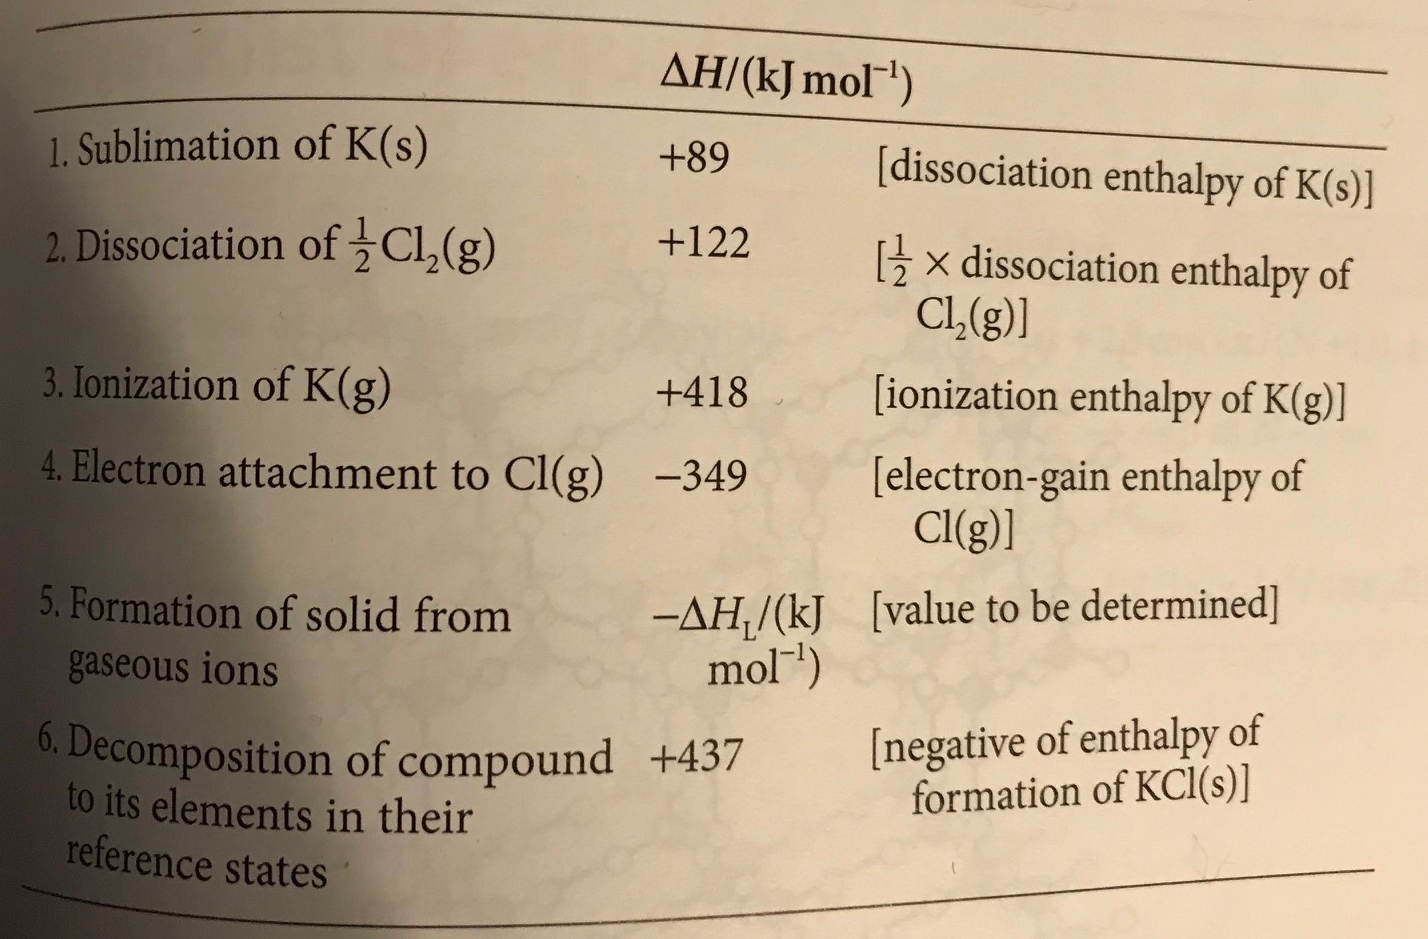
\includegraphics[scale=0.5]{res_ex2.png}
    %717 kj mol-1
    %exercici examen CaO (veure atkins)
    \end{exr}

\begin{exr}{}
Quin és el pH d'una dissolució de 0.1 M de clorur d'hidrogen? i d'una d'àcid benzoic a la mateixa concentració?
\end{exr}

\begin{exr}{}
Els productes de solubilitat de \ch{Fe(OH)3} i \ch{Zn(OH)2} són 4$\cdot$10$^{-38}$ i 4.5$\cdot$10$^{-17}$. A quin pH podem considerar que la precipitació de l'hidròxid de ferro és pràcticament completa mentre que l'ió \ch{Zn^{2+}} queda a una concentració de 0.5 M?
\end{exr}

\begin{exr}{}
Són reaccions REDOX
\[\ch{ClO- + NO2- <=> NO3- + Cl-} \]
\[\ch{2 CCl4 + K2CrO4 <=> 2 Cl2CO + CrO2Cl2 + 2 KCl} \]?
\end{exr}

\begin{exr}{}
Iguala la reacció \ch{H2O2 + I- <=> I2 + H2O}. Pista: quan hagis d'afegir hidrogen, fes-ho en forma de protons \ch{H+}.
\end{exr}

\begin{exr}{}
Iguala la reacció entre en benzaldehid i l'ió \ch{Cr2O7^{2-}} per donar àcid benzoïc i ió \ch{Cr^{+3}}. Pista: on calguin oxigens, afegeix molècules d'aigua; on calguin hidrogens, afegeix protons.
\end{exr}

\begin{exr}
Iguala la reacció \ch{ClO- + CrO2- <=> CrO4- + Cl-} en una dissolució bàsica. Pista: fes com sempre però al final tingues en compte que els reactius han d'incorporar l'ió \ch{OH-}.
\end{exr}
\begin{exr}
La reacció que té lloc en una bateria d'ió liti com la de la imatge
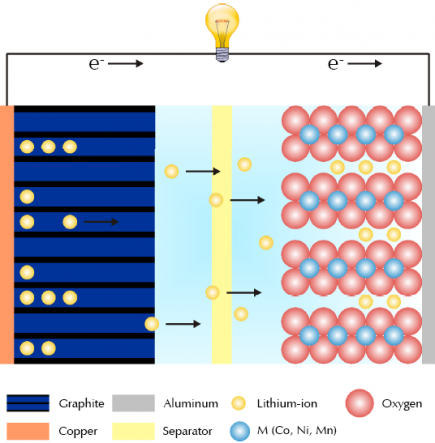
\includegraphics[scale=0.5]{LiIon.png}
és \ch{LiC6 + CoO2 <=> LiCoO2 + C6}. Escriu les dues mitges reaccions i fes-hi el balanç. Calcula el potencial de cel·la a partir de la $\Delta \varepsilon^{\circ}$ del \ch{Li+} (-3.0V) i del \ch{CoO2} (+1.1V).
Quins valors obtindries per a la reacció que tindria lloc en una bateria de Li i \ch{O2} ($\Delta \varepsilon^{\circ}$ de la reacció \ch{O2_{(g)} + 2 H+ + 2 e- -> H2O2_{(aq)}} és 0.3V).
\end{exr}

% \section{Forces intermoleculars}
% \begin{exr}
La ratio d'empaquetament d'una cel·la unitat es defineix com la fracció entre el volum omplert pels àtoms que la formen i el seu volum total. Calcula el RE de la cel·la unitat cúbica centrada en la cara i de la cel·la unitat cúbica centrada en el cos (veure Figura \ref{fig:crystal_structure}).
\end{exr}
\begin{exr}{}
Usant la descripció del Cicle de Born-Haber que trobaràs a la Wikipedia (\url{https://ca.wikipedia.org/wiki/Cicle_de_Born-Haber}) calcula l'energia reticular del Fluorur de Liti.
\end{exr}

\begin{exr}{}
Compara, per als diferents tipus de sòlids descrits, les següents característiques:
\begin{enumerate}
\item pressió de vapor
\item punt de fusió
\item punt d'ebullició
\item duresa
\item fragilitat
\item conducció elèctrica en estat sòlid
\item conducció elèctrica en estat líquid
\end{enumerate}
\end{exr}

\begin{exr}{}
El coure té una estructura cúbica de cara centrada, i l'aresta de la cel·la unitària és de 3.61${\AA}$. Pots suggerir algun tipus d'àtom que es pugui col·locar en els  intersticis de la seva xarxa sense distorsionar-la?
\end{exr}

\begin{exr}{}
Si la densitat del clorur sòdic sense defectes és de 2.165 g cm$^{-3}$, quina seria la densitat si tingués un ratio de 10$^{-3}$ defectes de a) Frenkel; b) Schottky. (el volum no varia amb els defectes)
\end{exr}

\begin{exr}
Explica, segons la teoria cinètico-molecular, la Figura \ref{fig:evap_vs_condens}. Com interpretes els termes \emph{equilibri dinàmic} i \emph{saturació}?
\end{exr}
\begin{exr}
És possible que un líquid arribi a estar sobreescalfat: temperatura superior a la d'ecullició per a aquella pressió però encara estat líquid, la qual cosa succeeix quan és molt pur i no hi ha partícules de pols.
Com aconseguiries que no es produeixi aquest sobreecalfament?
\end{exr} 
\begin{exr}
    Què ens produirà una cremada més gran: una massa $m$ d'\ch{H2O}(g) a 100 graus o la mateixa quantitat d'aigua líquida a la mateixa temperatura?
    \end{exr}
    
    \begin{exr}
    En un recipient hi ha aigua líquida. Es conecta el frecipient a una bomba de buit i es va abaixant la pressió sobre el líquid. Si la temperatura és de 60 graus, a quina pressió bullirà l'aigua?
    \end{exr}
    
    \begin{exr}
    Perquè a la Taula \ref{tab:pv} no apareix la $p_v$ de l'\ch{He}, \ch{H_2} i \ch{CH4}?
    \end{exr}
\begin{exr}
    Raona com canvia la $p_v$ d'una dissolució en funció de la seva concentració.
    \end{exr}
    
    \begin{exr}
    Determina la relació entre l'increment de pressió de vapor d'una dissolució i la fracció molar del solut.
    \end{exr}
    
    \begin{exr}
    La pressió de vapor de l'aigua a \qty{20}{\celsius} és \qty{17.54}{\mmHg}. Quan dissolem \qty{114}{\gram} de sucrosa en \qty{1000}{\gram} d'aigua, la pressió de vapor es redueix en \qty{0.11}{\mmHg}. Quin és el pes molecular de la sucrosa?
    \end{exr}
\begin{exr}
Quina és la constant de solubilitat del cromat d'argent (\ch{Ag2CrO4}) si la concentració d'una dissolució saturada d'aquesta sal té una concentració de 6.7$\times$10$^{-5}$M d'ions cromat?
\end{exr}
\begin{exr}{}
S'afegeix ió \ch{Ag+} a una dissolució que conté \ch{Cl-} i \ch{I-}, ambdós a una concentració de 0.01 M. Què precipita abans, \ch{AgCl} i \ch{AgI}. Quina és la concentració d'ions \ch{Ag+} quan la primera sal comença a precipitar? I quina és la concentració de l'anió del primer precipitat quan la segona sal comença a precipitar?
\end{exr}

\begin{exr}{}
Raona perquè per a una dissolució en la qual $\Delta H_{sol} <0$, un augment de la temperatura fa que la solubilitat disminueixi, i a l'inrevés.
\end{exr}

% \section{Controlant la temperatura}
% \begin{exr}
    Calcula el treball realitzat per comprimir un gas a pressió constant entre un volum inicial $V_1$ i un volum final $V_2$.
    \begin{center}
    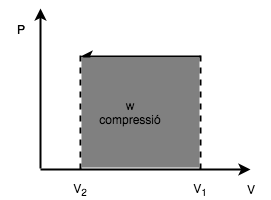
\includegraphics[scale=0.8]{wV.png}
    \end{center}
    \end{exr}
    \lct{}	
\begin{exr}{}
    Calcula el treball per dur un gas en un cilindre amb un èmbol des d'un estat de pressió 2 atm i volum 10 l fins a un estat de pressió 5 atm i volum 15 l per dos camins diferents:
    \begin{enumerate}
    \item Primer escalfant el gas a volum constant i després alliberant l'èmbol a pressió externa constant fins al volum desitjat.
    \item Segon deixant l'èmbol lliure (pressió externa constant) mentre escalfem el gas, seguit de continuar escalfant fins que arribem a la pressió objectiu.  
    \end{enumerate}
    \end{exr}

\begin{exr}{}
    \begin{itemize}
        \item Calcular el treball d'expansió reversible i isotèrmic, a \qty{25}{\celsius}, de \qty{3}{\mol} d'un gas ideal entre \qty{2}{\liter} i \qty{3}{\liter} de volum.
        \item I si es tracta d'un procés irreversible?
        \item Repeteix els dos apartats anteriors per a un procés de compressió entre \qty{3}{\liter} i \qty{2}{\liter} del mateix gas.
    \end{itemize}
    \end{exr}
    
 
\begin{exr}
A partir de l'expressió de l'energia cinètica mitja de les molècules d'un gas ideal, calcula l'energia de traslació que tindrà aquest gas a 298 K.
\end{exr}
\begin{exr}
Quina calor se li ha de donar a un gas ideal perquè s'expandeixi de manera reversible i isotèrmica de $V_1$ a $V_2$ ($V_2>V_1$)?
%l'energia interna només depèn de la temperatura. Per tant, aquí $\Delta U=0$. Per tant, $q=-w$ i podem integrar entre els dos volums per obtenir el resultat.
\end{exr}

\begin{exr}
\begin{center}
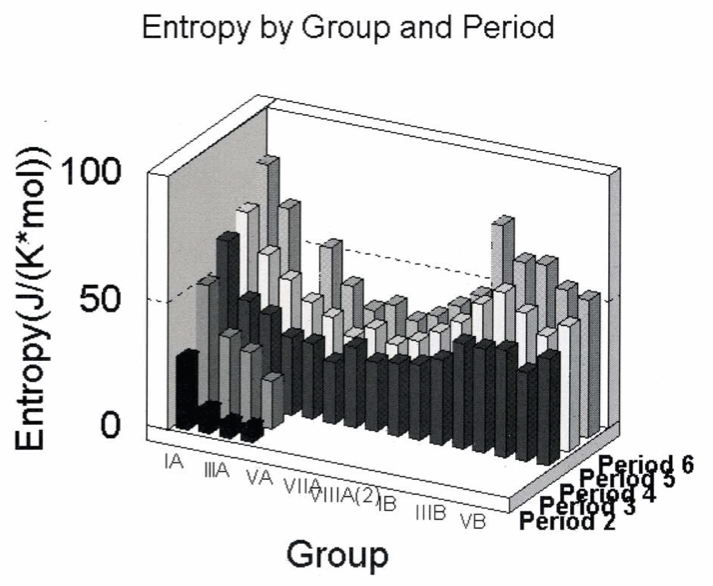
\includegraphics[scale=0.8]{EntropyPT.png}
\end{center}

La Figura mostra l'entropia normal $S^{\circ}_{298}$ per a elements de la taula periòdica, exclosos elements poliatòmics i que no formen sòlids.\cite{thoms_periodic_1995} Pots explicar:
\begin{enumerate}
\item perquè l'entropia augmenta en augmentar el període ($n$ més gran);
\item perquè l'entropia decreix al centre de cada període;i
\item quin és l'efecte d'un augmemnt de l'empaquetament o del grau de coordinació dels elements en l'entropia?
\end{enumerate}
\end{exr}
\begin{exr}
    Calcula l'energia lliure, l'entalpia i l'entropia normals per a la reacció \ch{3 H2_{(g)} + N2_{(g)} -> 2 NH3_{(g)}}. Què afavoreix i què desafavoreix la reacció? Succeiria igual a qualsevol temperatura?
    %\includegraphics[scale=0.8]{exdG.png}
    \end{exr}
\begin{exr}
Calcular els canvis d'energia lliure, entalpia i entropia per a la vaporització de l'aigua líquida. Quina influència hi té la pressió de vapor de l'aigua?
\end{exr}
\begin{exr}{}
Pots racionalitzar qualitativament els quatre factors implicats en la descripció de l'equilibri químic en les reaccions:
\[ \ch{H2_{(g)} <=> 2 H_{(g)}}\]
\[ \ch{H2_{(g)} + I2_{(g)} <=> 2 HI_{(g)}}\]?
Per a les dues reaccions, calcula el valor de $\Delta G^{\circ}$ a partir de dades obtingudes a la literatura (usa els enllaços de la Secció \ref{EnllacosInteres}).
\end{exr}

\begin{exr}{}
Com afectaria l'ús d'un catalitzador la corba d'energia lliure que hem dibuixat en el cas de la reacció de descomposició tèrmica del \ch{CaCO3}?
\end{exr}

\begin{exr}{}
Perquè podem usar la pressió de vapor enlloc de la concentració per a una substància gasosa en l'expressió de la constant d'equilibri?
Succeiria el mateix si el sistema no fos ideal? Serveix l'expressió per a qualsevol concentració de les substàncies reaccionants?
\end{exr}

\begin{exr}{}
Pots raonar perquè la constant d'equlibri de la descomposició tèrmica del \ch{CaCO3} és igual a $P_{\ch{CO2}}$?
\end{exr}

\begin{exr}{}
Com afecta la constant d'equilibri el fet d'igualar la reacció química amb coefficients que són els doble o el triple dels escrits inicialment?
\end{exr}

\begin{exr}
Quina és la relació entre la constant d'equilibri d'una reacció i la de la seva inversa?
\end{exr}
\begin{exr}
Escriu la constant d'equilibri de la reacció 
\[\ch{2 NO_{(g)} + O2_{(g)} <=> N2O4_{(g)}}\]
a partir de les de les reaccions 
\[\ch{2 NO_{(g)} + O2_{(g)} <=> 2 NO2_{(g)}}\]
i 
\[\ch{2 NO2_{(g)} + O2_{(g)} <=> N2O4_{(g)}}\]
\end{exr}
\begin{exr}
La constant d'equilibri de la reacció d'isomerització entre l'$n$-butà i l'isobutà és 2.5. Representa gràficament la tendència del sistema en funció de diverses concentracions inicials de cadascuna de les dues substàncies. (Pista: representa la pressió de vapor de l'$n$-butà en abcisses i la de l'isobutà en ordenades com mostra la Taula \ref{tab:Eqs}).
\end{exr}
\begin{exr}
    Fes una interpretació similar per al cas de la reacció de dissociació del sulfat de bari en els seus components iònics (veure Taula \ref{tab:Eqs}).
    \end{exr}
\begin{exr}{}
La constant d'equilibri de la dissociacio del \ch{NH4HS} sòlid en amoniac i sulfur d'hidrogen és de 0.11 atm$^2$. Si posem una mica d'aquest sòlid en un recipient tancat que conté amoniac a una pressió de 0.5 atm. Quina és la pressió final del sistema un cop assolit l'equlibri?
% pàgina 188 del mahan
\end{exr}

\begin{exr}
La constant d'equilibri de la reacció
\[
\ch{CO2_{(g)} + H2_{(g)} <=> CO_{(g)} + H2O_{(g)}}
\]
a 690K és 0.10. Quina és la pressió d'equilibri del sistema si barregem 0.5 mol de \ch{CO2} i 0.5 mol de \ch{H2} en un recipient de 5 l a 690K?
Si augmentéssim la T, la pressió augmentaria o disminuiria?
\end{exr}
\begin{exr}{}
Escriu la reacció àcid-base de l'ió carbonat en aigua en equlibri amb l'ió bicarbonat. Qui té el rol d'àcid i de base en la reacció directa i la inversa?
\end{exr}


% \section{Química de materials}
% \input{../Exercicis/compendi_GEAMaterials.tex}
% \section{Llum i química}
% \begin{exr}{}
Sabries explicar perquè la rotació en la molècula d'etilè (\ch{C2H4}) és més costosa energèticament que la rotació en la molècula d'età (\ch{C2H6})?
\end{exr}

\begin{exr}
La funció de Fermi $f(E)$ dóna la probabilitat de que un determinat estat energètic sigui ocupat a una determinada temperatura superior a 0K:
\[f(E)=\left( 1 + \exp \left[ \frac{E-E_f}{k_B T} \right] \right)^{-1}\]
a) Dibuixa $f(E)$. b) Si el nivell de Fermi per al coure és de 7eV, raona com es distribuiran els seus electrons a 0K i a 1000K.
\label{Ex:Fermi}.
\end{exr}  
\begin{exr}
Quants nodes té la funció $\psi(2s)$? i la $\psi(3s)$? i la $\psi(2p)$? 
\end{exr}
\begin{exr}
    A partir de la densitat de probabilitat podem preguntar-nos coses com on és el màxim de probabilitat (solucionant  $\frac{d D(r)}{dr}=0$) o bé calculant el valor promig de la distància de l'electró al nucli segons $<r>_{n,l}=\int_0^{\infty} r D(r)dr$. Mostra que $<r>_{2s}=\frac{6a_0}{Z}$ i $<r>_{2p}=\frac{5a_0}{Z}$ (veure Figura \ref{fig:D2s2p}).%Al tanto, no puc posar un marginnote dins d'un exr \marginnote{https://chemistry.stackexchange.com/questions/15208/difference-between-actual-position-of-electron-and-radial-distribution-probabili}
    \end{exr}
    \begin{exr}
        L'àtom de sodi es comporta de forma similar a l'àtom d'hidrogen pel que fa a la seva facilitat de "donar" un electró. Ho pots explicar en base a les densitats de probabilitat explicades a l'apartat anterior? Pensa en la llei de Coulomb i l'efecte pantalla dels electrons interiors.
        \end{exr}
        \begin{exr}
            Escriu la configuració electrònica de l'argó i del potassi. Perquè després d'omplir els orbitals 3p no omplim els orbitals 3d? Com raones que els metalls de transició de les  darreres columnes de la taula periòdica tinguin típicament valències de +2?
            \end{exr}
            \begin{exr}
                Pots explicar les dades de la Figura \ref{fig:AfinitatElectronica} en base a la configuració electrònica dels elements representats?
                \end{exr}
\printbibliography

\end{document}
